% Options for packages loaded elsewhere
\PassOptionsToPackage{unicode}{hyperref}
\PassOptionsToPackage{hyphens}{url}
\documentclass[
  10pt,
]{article}
\usepackage{xcolor}
\usepackage[margin=0.85in]{geometry}
\usepackage{amsmath,amssymb}
\setcounter{secnumdepth}{-\maxdimen} % remove section numbering
\usepackage{iftex}
\ifPDFTeX
  \usepackage[T1]{fontenc}
  \usepackage[utf8]{inputenc}
  \usepackage{textcomp} % provide euro and other symbols
\else % if luatex or xetex
  \usepackage{unicode-math} % this also loads fontspec
  \defaultfontfeatures{Scale=MatchLowercase}
  \defaultfontfeatures[\rmfamily]{Ligatures=TeX,Scale=1}
\fi
\usepackage{lmodern}
\ifPDFTeX\else
  % xetex/luatex font selection
\fi
% Use upquote if available, for straight quotes in verbatim environments
\IfFileExists{upquote.sty}{\usepackage{upquote}}{}
\IfFileExists{microtype.sty}{% use microtype if available
  \usepackage[]{microtype}
  \UseMicrotypeSet[protrusion]{basicmath} % disable protrusion for tt fonts
}{}
\makeatletter
\@ifundefined{KOMAClassName}{% if non-KOMA class
  \IfFileExists{parskip.sty}{%
    \usepackage{parskip}
  }{% else
    \setlength{\parindent}{0pt}
    \setlength{\parskip}{6pt plus 2pt minus 1pt}}
}{% if KOMA class
  \KOMAoptions{parskip=half}}
\makeatother
\usepackage{longtable,booktabs,array}
\newcounter{none} % for unnumbered tables
\usepackage{calc} % for calculating minipage widths
% Correct order of tables after \paragraph or \subparagraph
\usepackage{etoolbox}
\makeatletter
\patchcmd\longtable{\par}{\if@noskipsec\mbox{}\fi\par}{}{}
\makeatother
% Allow footnotes in longtable head/foot
\IfFileExists{footnotehyper.sty}{\usepackage{footnotehyper}}{\usepackage{footnote}}
\makesavenoteenv{longtable}
\usepackage{graphicx}
\usepackage{placeins}
\makeatletter
\newsavebox\pandoc@box
\newcommand*\pandocbounded[1]{% scales image to fit in text height/width
  \sbox\pandoc@box{#1}%
  \Gscale@div\@tempa{\textheight}{\dimexpr\ht\pandoc@box+\dp\pandoc@box\relax}%
  \Gscale@div\@tempb{\linewidth}{\wd\pandoc@box}%
  \ifdim\@tempb\p@<\@tempa\p@\let\@tempa\@tempb\fi% select the smaller of both
  \ifdim\@tempa\p@<\p@\scalebox{\@tempa}{\usebox\pandoc@box}%
  \else\usebox{\pandoc@box}%
  \fi%
}
% Set default figure placement to htbp
\def\fps@figure{htbp}
\makeatother
\setlength{\emergencystretch}{3em} % prevent overfull lines
\providecommand{\tightlist}{%
  \setlength{\itemsep}{0pt}\setlength{\parskip}{0pt}}
\usepackage{bookmark}
\IfFileExists{xurl.sty}{\usepackage{xurl}}{} % add URL line breaks if available
\urlstyle{same}
\hypersetup{
  pdftitle={Supplementary Evidence for the Corrected CI Decision Simulation},
  pdfauthor={Abishek Kumar Giri},
  hidelinks,
  pdfcreator={LaTeX via pandoc}}

\title{Supplementary Evidence for the Corrected CI Decision Simulation}
\author{Abishek Kumar Giri}
\date{6 September 2026}

\begin{document}
\maketitle

\section{Scope}\label{scope}

This supplement replaces all numerical tables and figures from the
original submission. The source-of-truth file and machine-readable
artifacts define the corrected numerical record. Original materials are
retained under review/original. These are simulation experiments, not
causal release-cost estimates.

\section{Full replay conditions}\label{full-replay-conditions}

\subsection{artificial default delay}\label{artificial-default-delay}

\par\medskip\noindent\begin{minipage}{\linewidth}\centering
\begin{tabular}{@{}llll@{}}
\toprule\noalign{}
Policy & Mean cost & Sample SD & 95\% seed CI \\
\midrule\noalign{}
Always block & 1,865 & 0 & 1,865 to 1,865 \\
Always canary & 2,020 & 0 & 2,020 to 2,020 \\
Always deploy & 2,900 & 0 & 2,900 to 2,900 \\
Bayesian rate & 1,713 & 0 & 1,713 to 1,713 \\
Rolling cost rule & 2,085 & 0 & 2,085 to 2,085 \\
Heuristic & 2,288 & 0 & 2,288 to 2,288 \\
LinUCB & 1,877.5 & 0 & 1,877.5 to 1,877.5 \\
Bias-only LinUCB & 1,735 & 0 & 1,735 to 1,735 \\
LinUCB wrapper & 1,877.5 & 0 & 1,877.5 to 1,877.5 \\
Static rules & 1,929 & 0 & 1,929 to 1,929 \\
Thompson & 1,889.6 & 52.9 & 1,871 to 1,908.7 \\
\bottomrule
\end{tabular}
\end{minipage}\par\medskip

\subsection{online smoke}\label{online-smoke}

\par\medskip\noindent\begin{minipage}{\linewidth}\centering
\begin{tabular}{@{}llll@{}}
\toprule\noalign{}
Policy & Mean cost & Sample SD & 95\% seed CI \\
\midrule\noalign{}
Always block & 1,865 & 0 & 1,865 to 1,865 \\
Always canary & 2,020 & 0 & 2,020 to 2,020 \\
Always deploy & 2,900 & 0 & 2,900 to 2,900 \\
Bayesian rate & 1,713.5 & 0 & 1,713.5 to 1,713.5 \\
Rolling cost rule & 1,970.5 & 0 & 1,970.5 to 1,970.5 \\
Heuristic & 2,325 & 0 & 2,325 to 2,325 \\
LinUCB & 1,863 & 0 & 1,863 to 1,863 \\
Bias-only LinUCB & 1,739 & 0 & 1,739 to 1,739 \\
LinUCB wrapper & 1,863 & 0 & 1,863 to 1,863 \\
Static rules & 1,884 & 0 & 1,884 to 1,884 \\
Thompson & 1,857.1 & 62.6 & 1,835.2 to 1,878.5 \\
\bottomrule
\end{tabular}
\end{minipage}\par\medskip

\subsection{real github actions}\label{real-github-actions}

\par\medskip\noindent\begin{minipage}{\linewidth}\centering
\begin{tabular}{@{}llll@{}}
\toprule\noalign{}
Policy & Mean cost & Sample SD & 95\% seed CI \\
\midrule\noalign{}
Always block & 1,027 & 0 & 1,027 to 1,027 \\
Always canary & 836 & 0 & 836 to 836 \\
Always deploy & 860 & 0 & 860 to 860 \\
Bayesian rate & 669 & 0 & 669 to 669 \\
Rolling cost rule & 624.5 & 0 & 624.5 to 624.5 \\
Heuristic & 860 & 0 & 860 to 860 \\
LinUCB & 779 & 0 & 779 to 779 \\
Bias-only LinUCB & 650 & 0 & 650 to 650 \\
LinUCB wrapper & 779 & 0 & 779 to 779 \\
Static rules & 640 & 0 & 640 to 640 \\
Thompson & 665.7 & 39.8 & 652.1 to 680.1 \\
\bottomrule
\end{tabular}
\end{minipage}\par\medskip

\subsection{robustness high failure}\label{robustness-high-failure}

\par\medskip\noindent\begin{minipage}{\linewidth}\centering
\begin{tabular}{@{}llll@{}}
\toprule\noalign{}
Policy & Mean cost & Sample SD & 95\% seed CI \\
\midrule\noalign{}
Always block & 1,865 & 0 & 1,865 to 1,865 \\
Always canary & 3,180 & 0 & 3,180 to 3,180 \\
Always deploy & 5,800 & 0 & 5,800 to 5,800 \\
Bayesian rate & 1,865 & 0 & 1,865 to 1,865 \\
Rolling cost rule & 2,425.5 & 0 & 2,425.5 to 2,425.5 \\
Heuristic & 4,115 & 0 & 4,115 to 4,115 \\
LinUCB & 1,972 & 0 & 1,972 to 1,972 \\
Bias-only LinUCB & 1,905 & 0 & 1,905 to 1,905 \\
LinUCB wrapper & 1,972 & 0 & 1,972 to 1,972 \\
Static rules & 2,578 & 0 & 2,578 to 2,578 \\
Thompson & 1,955.8 & 27.2 & 1,946.1 to 1,965.5 \\
\bottomrule
\end{tabular}
\end{minipage}\par\medskip

\subsection{robustness long delay}\label{robustness-long-delay}

\par\medskip\noindent\begin{minipage}{\linewidth}\centering
\begin{tabular}{@{}llll@{}}
\toprule\noalign{}
Policy & Mean cost & Sample SD & 95\% seed CI \\
\midrule\noalign{}
Always block & 1,865 & 0 & 1,865 to 1,865 \\
Always canary & 2,020 & 0 & 2,020 to 2,020 \\
Always deploy & 2,900 & 0 & 2,900 to 2,900 \\
Bayesian rate & 1,713 & 0 & 1,713 to 1,713 \\
Rolling cost rule & 2,077 & 0 & 2,077 to 2,077 \\
Heuristic & 2,319 & 0 & 2,319 to 2,319 \\
LinUCB & 1,973 & 0 & 1,973 to 1,973 \\
Bias-only LinUCB & 1,777.5 & 0 & 1,777.5 to 1,777.5 \\
LinUCB wrapper & 1,973 & 0 & 1,973 to 1,973 \\
Static rules & 1,924 & 0 & 1,924 to 1,924 \\
Thompson & 1,917 & 61.6 & 1,895.5 to 1,939.3 \\
\bottomrule
\end{tabular}
\end{minipage}\par\medskip

\subsection{robustness low block}\label{robustness-low-block}

\par\medskip\noindent\begin{minipage}{\linewidth}\centering
\begin{tabular}{@{}llll@{}}
\toprule\noalign{}
Policy & Mean cost & Sample SD & 95\% seed CI \\
\midrule\noalign{}
Always block & 1,005 & 0 & 1,005 to 1,005 \\
Always canary & 2,020 & 0 & 2,020 to 2,020 \\
Always deploy & 2,900 & 0 & 2,900 to 2,900 \\
Bayesian rate & 1,005 & 0 & 1,005 to 1,005 \\
Rolling cost rule & 1,273.5 & 0 & 1,273.5 to 1,273.5 \\
Heuristic & 2,325 & 0 & 2,325 to 2,325 \\
LinUCB & 1,072 & 0 & 1,072 to 1,072 \\
Bias-only LinUCB & 1,024 & 0 & 1,024 to 1,024 \\
LinUCB wrapper & 1,072 & 0 & 1,072 to 1,072 \\
Static rules & 1,591 & 0 & 1,591 to 1,591 \\
Thompson & 1,069.6 & 20 & 1,062.8 to 1,076.9 \\
\bottomrule
\end{tabular}
\end{minipage}\par\medskip

\subsection{robustness short delay}\label{robustness-short-delay}

\par\medskip\noindent\begin{minipage}{\linewidth}\centering
\begin{tabular}{@{}llll@{}}
\toprule\noalign{}
Policy & Mean cost & Sample SD & 95\% seed CI \\
\midrule\noalign{}
Always block & 1,865 & 0 & 1,865 to 1,865 \\
Always canary & 2,020 & 0 & 2,020 to 2,020 \\
Always deploy & 2,900 & 0 & 2,900 to 2,900 \\
Bayesian rate & 1,714.5 & 0 & 1,714.5 to 1,714.5 \\
Rolling cost rule & 1,949 & 0 & 1,949 to 1,949 \\
Heuristic & 2,294 & 0 & 2,294 to 2,294 \\
LinUCB & 1,950 & 0 & 1,950 to 1,950 \\
Bias-only LinUCB & 1,750 & 0 & 1,750 to 1,750 \\
LinUCB wrapper & 1,950 & 0 & 1,950 to 1,950 \\
Static rules & 1,853.5 & 0 & 1,853.5 to 1,853.5 \\
Thompson & 1,909.6 & 51.3 & 1,891.8 to 1,927.9 \\
\bottomrule
\end{tabular}
\end{minipage}\par\medskip

\section{Page Hinkley calibration}\label{page-hinkley-calibration}

Fixed deploy, IID failure labels, 1,150 observations, seeds 1000-1029.
The selected threshold is 400; selection criterion is no more than 10\%
of streams with any alarm in each of two null cells. This finite-sample
screen is not a theoretical error bound.

\par\medskip\noindent\begin{minipage}{\linewidth}\centering
\begin{tabular}{@{}llll@{}}
\toprule\noalign{}
Threshold & Failure rate & Mean alarms & Fraction with any alarm \\
\midrule\noalign{}
20 & 0.1 & 14.9 & 1.000 \\
20 & 0.35 & 26.5 & 1.000 \\
50 & 0.1 & 3.5 & 0.967 \\
50 & 0.35 & 8.5 & 1.000 \\
100 & 0.1 & 0.7 & 0.533 \\
100 & 0.35 & 2.2 & 0.867 \\
200 & 0.1 & 0 & 0.000 \\
200 & 0.35 & 0.4 & 0.367 \\
400 & 0.1 & 0 & 0.000 \\
400 & 0.35 & 0 & 0.033 \\
800 & 0.1 & 0 & 0.000 \\
800 & 0.35 & 0 & 0.000 \\
\bottomrule
\end{tabular}
\end{minipage}\par\medskip

\section{Drift evaluation}\label{drift-evaluation}

Mean cumulative expected pseudo-regret uses all 500 decisions. Realized
costs exclude a common censored-delay mask. Terminal observations are
included in cost evaluation but not in model learning. The moment-rate
control accounts for the synthetic canary multiplier; CI replay controls
assume an action-independent label.

\par\medskip\noindent\begin{minipage}{\linewidth}\centering
\begin{tabular}{@{}llll@{}}
\toprule\noalign{}
Policy & Stationary & Abrupt & Gradual \\
\midrule\noalign{}
Static rules & 77.1 & 88.3 & 94.7 \\
LinUCB & 53.5 & 65.1 & 68.1 \\
Thompson & 66.9 & 70.8 & 79.5 \\
PH threshold 50 & 55 & 76.8 & 71.2 \\
PH threshold 400 & 53.5 & 65.1 & 68.1 \\
Scalar moment rate & 23.2 & 163.1 & 73.8 \\
Rate window 50 & 34.1 & 47.5 & 36.4 \\
Rate window 100 & 31.5 & 64.6 & 34.7 \\
\bottomrule
\end{tabular}
\end{minipage}\par\medskip

\begin{figure}
\centering
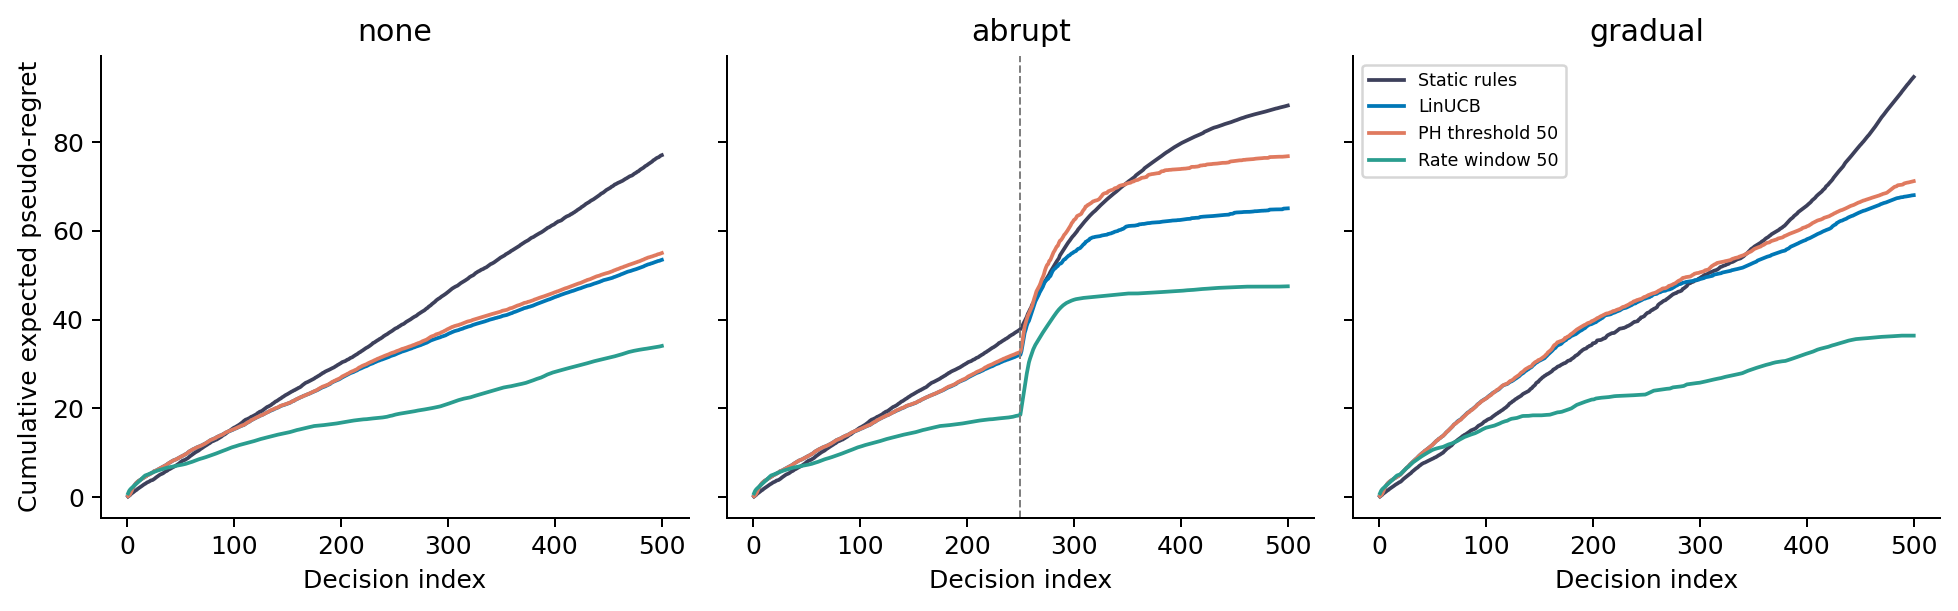
\includegraphics[width=0.95\linewidth,height=\textheight,keepaspectratio,alt={Expected pseudo-regret by decision index}]{../figures/fig_drift_recovery_curves.png}
\caption{Expected pseudo-regret by decision index}
\end{figure}

\begin{figure}
\centering
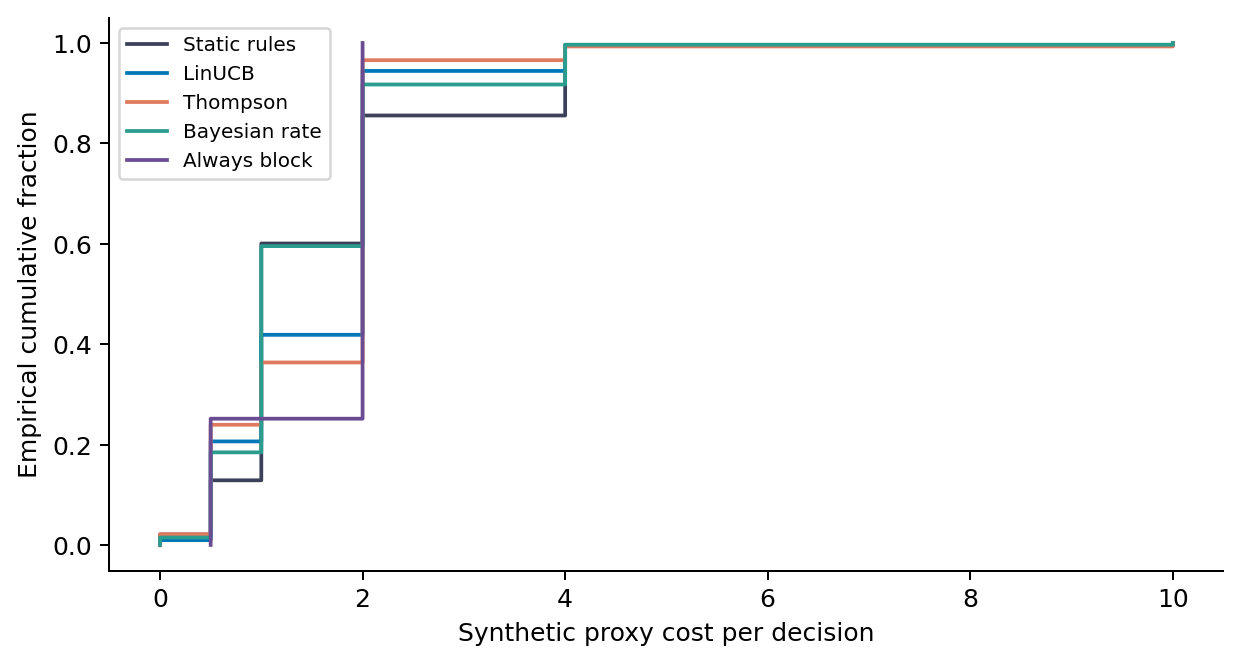
\includegraphics[width=0.95\linewidth,height=\textheight,keepaspectratio,alt={Empirical synthetic cost distribution}]{../figures/fig_cost_cdf_per_step.png}
\caption{Empirical synthetic cost distribution}
\end{figure}

\begin{figure}
\centering
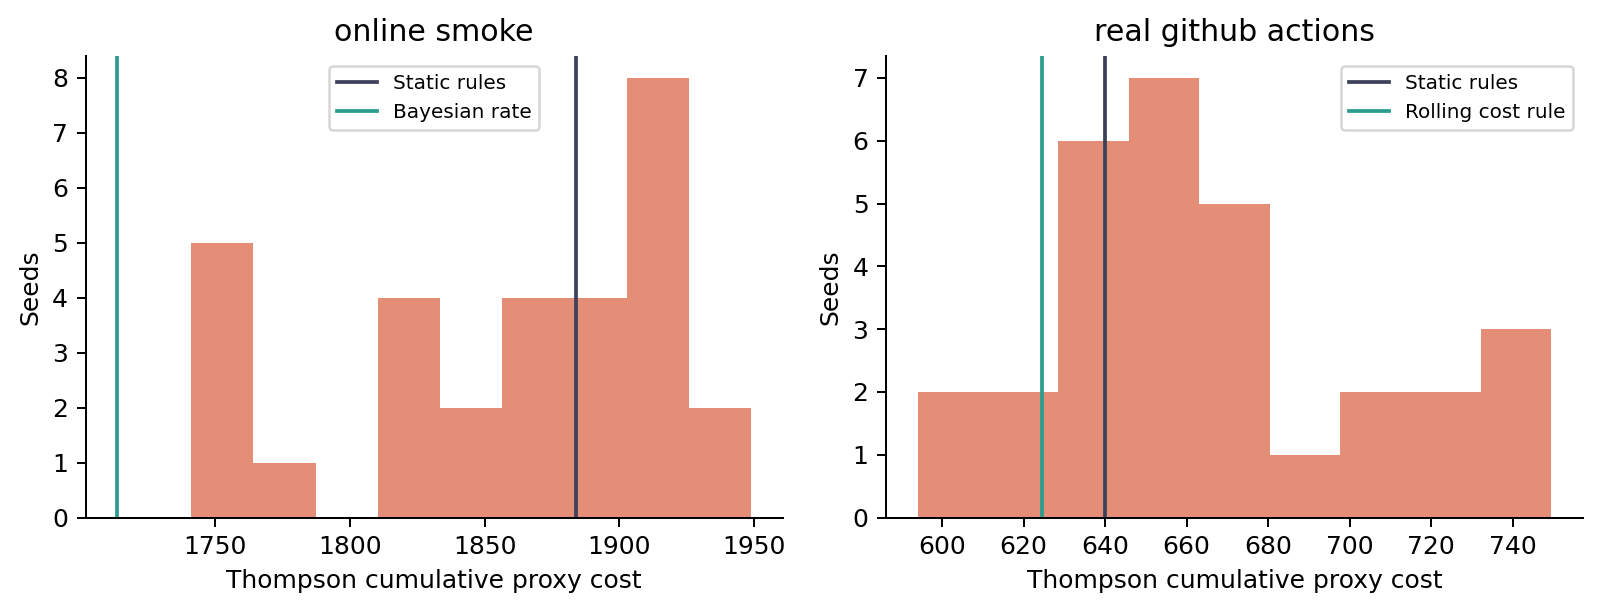
\includegraphics[width=0.95\linewidth,height=\textheight,keepaspectratio,alt={Thompson seed costs and simple comparators}]{../figures/fig_thompson_seed_distribution.png}
\caption{Thompson seed costs and simple comparators}
\end{figure}

\begin{figure}
\centering
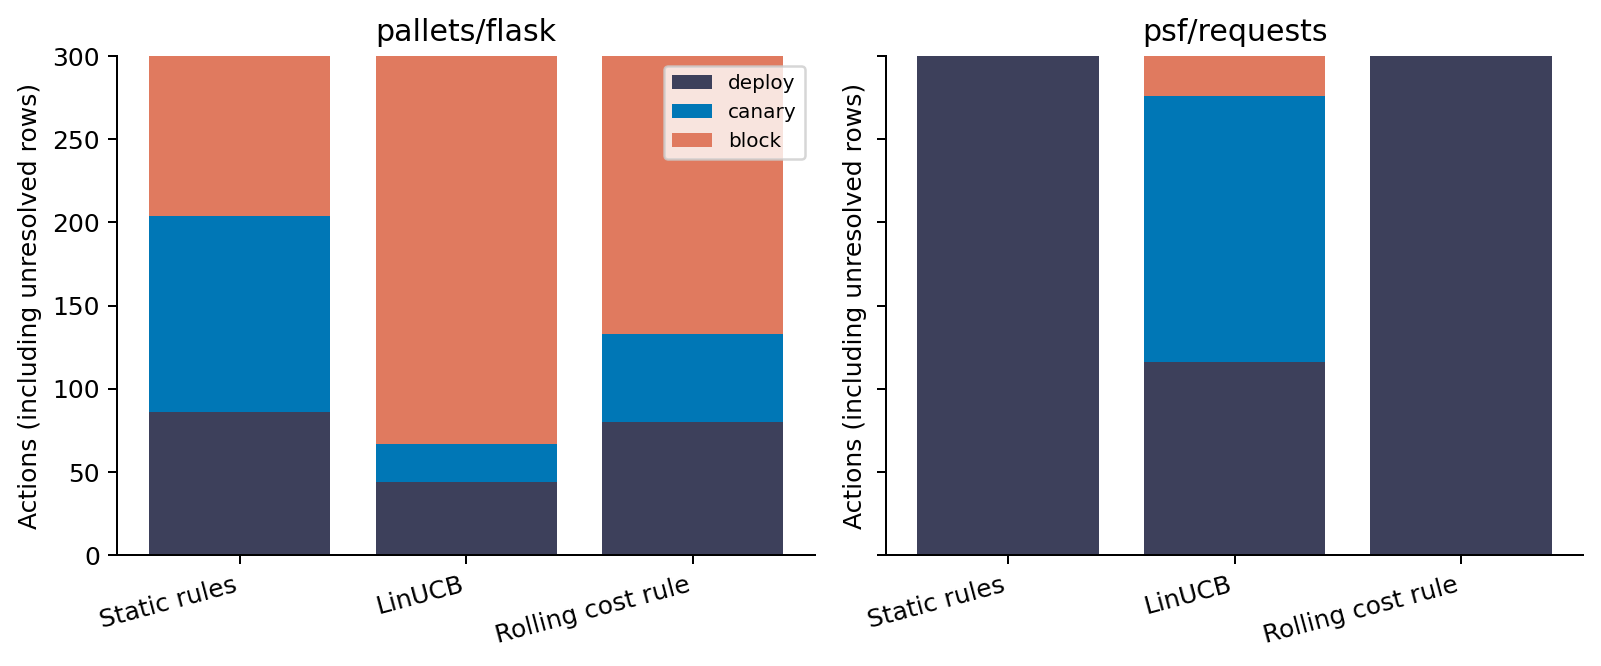
\includegraphics[width=0.95\linewidth,height=\textheight,keepaspectratio,alt={Project-local real-data action counts}]{../figures/fig_action_distribution.png}
\caption{Project-local real-data action counts}
\end{figure}

\begin{figure}
\centering
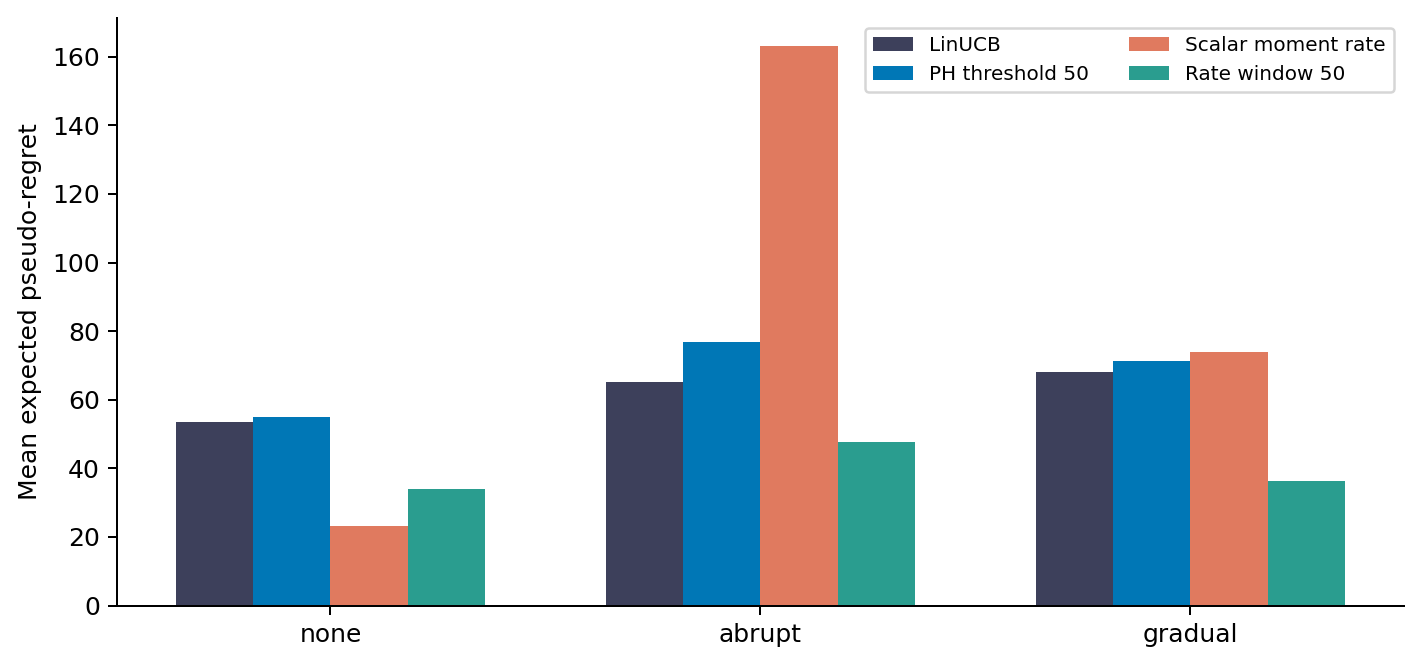
\includegraphics[width=0.95\linewidth,height=\textheight,keepaspectratio,alt={Expected pseudo-regret across drift modes}]{../figures/fig_drift_mode_bars.png}
\caption{Expected pseudo-regret across drift modes}
\end{figure}

\begin{figure}
\centering
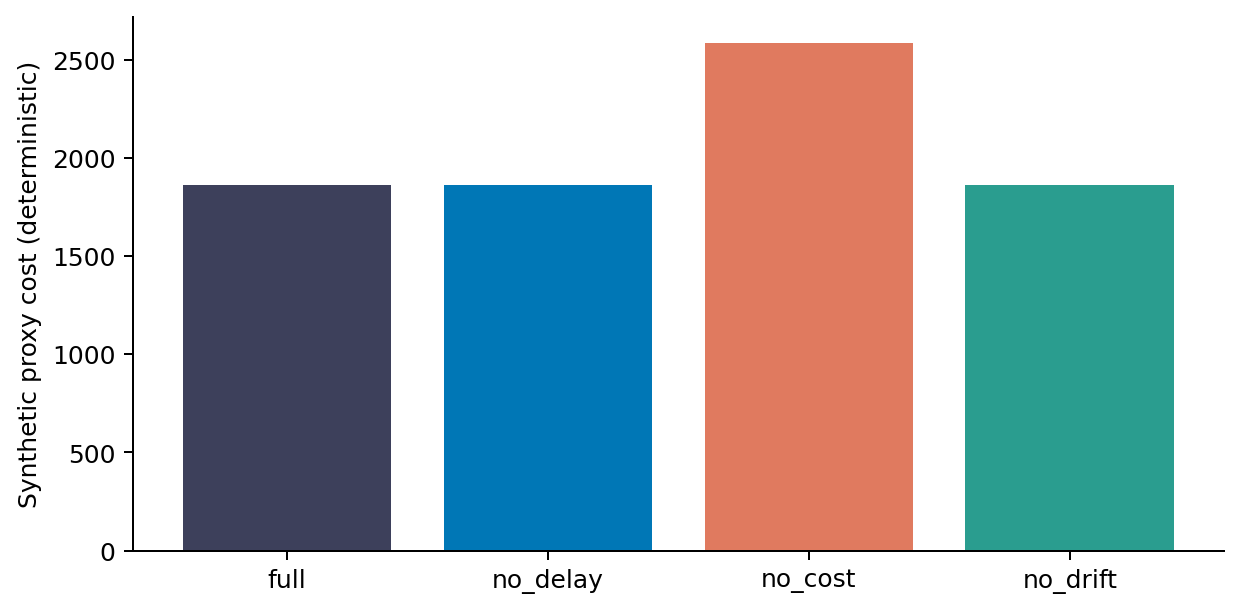
\includegraphics[width=0.95\linewidth,height=\textheight,keepaspectratio,alt={Corrected deterministic ablation costs}]{../figures/fig_ablation_bars.png}
\caption{Corrected deterministic ablation costs}
\end{figure}

\FloatBarrier
\section{Reproducibility}\label{reproducibility}

Run the commands in the root README from a clean checkout. The frozen
CSV hashes and code hashes are in corrected/manifest.json. This run used
Python 3.13 and the exact dependency versions in requirements-audit.txt.
The main build scripts use Pandoc and a TeX installation.

\section{Remaining limitations}\label{remaining-limitations}

The synthetic fixture generator is unavailable. The real export lacks
collection provenance and workflow identities; it cannot be interpreted
as independent deployment decisions. Deterministic policy repetition
does not supply dataset uncertainty. Hyperparameter sensitivity is
exploratory on the same export. Real opportunity costs, deployment
incidents, action-dependent censoring and policy effects on future
releases are unmeasured. The original empirical operating-boundary claim
is withdrawn.

\end{document}
